\subsubsection{UC18 - Debug della generazione del \glossario{prompt}}\label{UC18}

\begin{figure}[H]
  \centering
  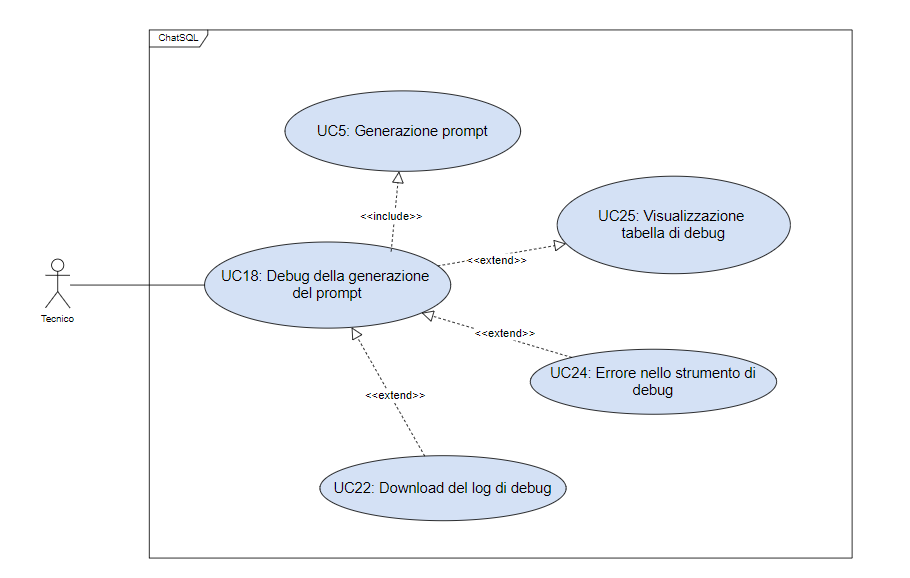
\includegraphics[width=0.90\textwidth]{assets/uc18.png}
  \caption{UC18}
\end{figure}


\paragraph*{Descrizione}
Il Tecnico vuole poter testare il \glossario{prompt} generato e interroga il sistema per comprendere la corretta formattazione del \glossario{dizionario dati}. Visualizza una tabella contenente i campi del \glossario{dizionario dati} e lo score ottenuto per questi.

\paragraph*{Attori principali}
Tecnico

\paragraph*{Precondizioni}
\begin{itemize}
  \item Il Tecnico è correttamente autenticato tramite login (\hyperref[UC1]{UC1});
  \item È presente almeno un \glossario{dizionario dati} nel sistema;
  \item Il Tecnico inserisce una richiesta in linguaggio naturale (\hyperref[UC3]{UC3});
  \item Il sistema genera il \glossario{prompt} (\hyperref[UC5]{UC5});
  \item Il Tecnico seleziona lo strumento di debug.
\end{itemize}

\paragraph*{Postcondizioni}
\begin{itemize}
  \item Il sistema genera un \glossario{log};
  \item Il sistema genera una tabella dei migliori risultati individuati;
\end{itemize}

\paragraph*{Scenario principale}
\begin{enumerate}
  \item Il Tecnico riceve il \glossario{prompt} dal sistema (\hyperref[UC5]{UC5});
  \item Il Tecnico seleziona lo strumento di debug;
  \item Lo strumento di debug genera una tabella dei risultati individuati dal sistema; 
  \item Lo strumento di debug genera un \glossario{log} descrittivo dei passaggi per la composizione del \glossario{prompt}.  
\end{enumerate}

\paragraph*{Inclusioni}
\begin{itemize}
  \item Generazione \glossario{prompt}.
\end{itemize}

\paragraph*{Estensioni}
\begin{itemize}
  \item Errore nello strumento di debug (\hyperref[UC24]{UC24});
  \item Download del log di debug (\hyperref[UC22]{UC22});
  \item Visualizzazione della tabella di debug (\hyperref[UC25]{UC25}).
\end{itemize}